\chapter{Tone}

This chapter describes the phonological characteristics of tone in Moro and regular phonological processes which apply to it. Additional processes involving tone which involve particular affixes are described throughout the grammar.

Moro contrasts two tones, high and low. Tonal minimal pairs are provided in Table \ref{tab:ch4:1}. High tone is marked with an accent \'{}, whereas low tone is unmarked. This transcription also reflects the distribution and behavior of the tones. High tone can be spread, shifted and trigger downstep in the case of adjacent H tones, whereas low tone is inert. 

\begin{table}
  \begin{tabular}{lp{1.5in}lp{1.5in}}
    \lsptoprule
  \multicolumn{4}{c}{HH vs. LH} \\
ɽŕwɜ́	&	‘goat dung’	&	ɽrwɜ́	&	‘testicle’	\\
ðólóŋ	&‘iron nail’	&	ðolóŋ	&	‘eel’			\\
wáɾá	&‘chicken’		&	waɾá	&	‘baobab tree’\\
\midrule
  \multicolumn{4}{c}{LL vs. LH} \\
ŋəwa	&	‘young girl’&	ŋəwá	& ‘youth (girls), virginity, purity’ \\
eða		&‘meat’			&	eðá		&	‘why?’ \\
ŋata	&‘dirtiness’	&ŋatá		&	‘very little’\\
\midrule
  \multicolumn{4}{c}{HL vs. LH} \\
káwːa	&‘s/he is urinating’ &	kawːá	&	‘s/he is persuading’\\
ðwála	&‘height’		&	ðwalá	&	‘it is tall (ð noun class)\\
\midrule
  \multicolumn{4}{c}{HL vs. HH} \\
ðóla	&‘rat’			&	ŋólá	& 	‘tears’\\
\midrule
  \multicolumn{4}{c}{HL vs. LL} \\
ðóla	&‘rat’			&	ola		&	‘large covered gourd for milk’\\
\midrule
  \multicolumn{4}{c}{LL(L) vs. HH(H)} \\
ləmeə	&‘flea’			&	lə́méə	&	‘bear-like animal’\\
ðəɾa	&‘tree sp.'		&	ðə́ɾá	& ‘vine of gourd’\\
lwata	&‘bat for threshing, beating grain; hoof of camel’	& lwátá	&	‘area for a dance, stick-fighting’\\
ŋaləŋa	&‘song’			&	ŋálə́ŋá	&	‘kingdom’	\\
\lspbottomrule 
  \end{tabular}
  \caption{Tone minimal pairs and near minimal pairs}
  \label{tab:ch4:1}
\end{table}

Perfect minimal pairs contrasting HL with LL or HL with HH have not been noted. Forms that differ by tone and the initial consonant are included here. This may be a gap due to the lower frequency of HL words.  There are no tonal minimal pairs for verbs or adjectives, as the distribution of tone on verbs and adjectives is morphologically and prosodically determined, as described for verbs in Chapter \ref{chapter:verbs}, particularly in Section \ref{section:defaulttone}, and for adjectives in Section \ref{section:adjective}.

\section{Tone bearing units}
Tone bearing units are vowels, but high tone can also appear on nasals and [r] when these are syllabic or occur in a coda. In other positions, the consonants are always low-toned. Nevertheless, there are restrictions on the distribution of high tones on the sonorant consonants. 

\subsection{Nasal tone bearing units}	 	
Nasals can bear high tone in word-initial position when followed by a consonant. Contrasts between low-toned and high-toned nasals in this position are observed for [nd] and [ŋg] sequences:
	
\ea	 	
\begin{tabular}[t]{llll}
 ḿbú	&‘go!’  & {}& {}  \\
ńdró	&‘sleep!’	&		ndá	&‘head’  \\
 ŋ́gú	&{‘alcoholic drink’}	&ŋɡáɾá	&‘salt’\\
ŋ́gá	&‘urine’ & {} & {} \\
\end{tabular}
	\z

Nasals in coda position are low-toned, both medially and word-finally, even if the preceding vowel bears high tone:

\ea 	\begin{tabular}[t]{llll}
  \multicolumn{2}{l}{Word-internal} &   \multicolumn{2}{l}{Word-final} \\
\midrule
ebamba		&	‘drum’			&	etám	&	‘neck’ \\
ondəðéa		&‘lice (on humans)’	&ŋgón		&	‘squirrel’ \\
ðə́púndŕí	&‘wooden object’	&	ŋgáɲ	& ‘sickness’ \\
lə́ŋɡə́ŋé		&‘bell’				&	ɽdóŋ	&‘pointy back of head’ \\
			 	\end{tabular} \z

There is one exception to this pattern in the verb system. Consider the following verbs, conjugated in the proximal imperative and the proximal imperfective, which show a three-way distinction for how nasal-stop sequences are treated with respect to tone. The general grammatical tone pattern for the proximal imperative is that all tone-bearing units are high-toned. The general grammatical tone pattern for the proximal imperfective is that H tone is placed on the first tone-bearing unit, and may spread to a second if the syllable is not closed. If the root begins with a consonant cluster, H tone is placed on the preceding vocalic prefix.

\ea 	\begin{tabular}[t]{llll}
&	Proximal &  Proximal &	 \\
&	Imperative	&Imperfective	&		\\
\midrule
a.	&	ńdrát̪-ó	&	k-a-ńdrat̪-a		&‘be near to’\\
b.	&	ńdr-ó	&	k-a-ńdr-a		&‘sleep’\\
c.	&	ŋgát̪-ó	&	k-a-ŋgát̪-eə		&‘go away, leave’\\
d.	&	ŋɡít̪-ú	&	k-ɜ́-ŋɡit̪-iə		&‘let, allow’\\
	\end{tabular}\z

In each of these cases, the nasal-consonant sequence is root-initial, as shown by the imperative form, which consists of the verb root and a suffix \textit{-ó}. This is the position that allows nasals to bear H tone. The first two verbs have high tone on the nasal, but the second two do not. In the imperfective form, the first two verbs have high tone on the nasal, which does not spread. This indicates that the nasal functions as the coda, creating a heavy syllable that prevents further tone spreading. In [c], H tone skips the nasal and appears instead on the first vowel of the root. In [d], the H tone appears on the vowel preceding the root rather than on the first vowel of the root. The nasal-consonant sequence in (4)c may be a prenasalized stop, since it is ignored in terms of tone assignment. The pattern in [d] occurs when initial geminate consonants are followed by a vowel in the root: (\textit{g-á-w:aðat̪-a} ‘s/he finds’), indicating that this form is a true NC sequence. 

	% TODO Sharon One test is their pattern in reduplication. 

\subsubsection{Liquid (l and r) tone bearing units}	 
Although the trill [r] can appear word-initially preceding a consonant, there are no attestations of it bearing high tone in that position. However, word-medially [r] can appear in either C \underline{\hspace{0.3cm}} V or C\underline{\hspace{0.4cm}} C environments, and can bear tone in these cases:

\ea
\begin{tabular}[t]{llllp{3.25cm}}
 & Low-toned & & High-toned\\
\midrule
\# \underline{\hspace{0.3cm}} C &	rða		&	‘meat’\\
C \underline{\hspace{0.3cm}} C 	&	brlágá	&	‘slime’		&	kŕmɜ́ʧú	&	‘quieten s.o.!’\\
C \underline{\hspace{0.3cm}} V	&	ɜbəlúkriə	&	‘dove’	&	ɜ́tŕiə́	&	‘gum of mouth’\\

&&&ɽŕóðéə	&	‘coccyx’\\
&&&ɜlíbŕiɜ	&	‘thread’\\
&&&ðəbət̪ŕʷá	&	‘(shield made from) palm frond’\\
\end{tabular}
\z

It is not clear what the syllable structure of these forms is. As the consonant sequence involves a rise in sonority from the stop or flap to [r], this could be construed as an onset. Some words can begin with stop-r sequences. However, it may be that an underlying [ə] vowel has been dropped, with its high tone transferred to the [r], so /ɜ́tə́riə́/  $\rightarrow$ [ɜ́tŕiə́]. In slow speech, there is often an [ə].

When [r] appears in coda position followed by a less-sonorant consonant, it can also bear H tone, but only if the preceding vowel is high-toned. 

\ea
\begin{tabular}[t]{lll}
áŕ	&	ŋáŕlá	&	‘spear’	\\
ar	&	ŋarléðá	&	‘dirt’	\\
ár	&	evárt̪ə́ŋé	&	‘tree sp.’\\
\end{tabular}
\z

In word-final position, however, [r] is always low-toned. This is the same pattern as with the nasals. 

\ea
\begin{tabular}[t]{ll}
ðoɽár		&	‘snake sp. (yellow, white)\\
ðəwə́r		&	‘spring (water)’\\
ləpér		&	‘tail’\\
əltúr		&	‘umbilical hernia’\\
luŋwur		&	‘small bowl’\\
vələðar		&	‘pull (from here to there)!\\
\end{tabular}
\z

As for [l], it typically bears low tone, even if the preceding vowel is high.When geminate, it is also low-toned.
\ea
\begin{tabular}[t]{ll}
ortʃəl	&	‘poisonous tree’\\
ŋwol	&	‘sound, tears’\\
logə́l	&	‘eagle’\\
eɾél	&	‘side of face’\\
lːoá	&	‘elbow’\\
\end{tabular}
\z

[l] can occasionally bear high tone when in coda position, but only if the vowel following it has been deleted and the [l] recuperates the vowel’s tone, a case of tonal stability. For example, the 3pl object marker \textit{-lo} can reduce or delete its vowel before the instrumental \textit{-ja}. 
	% TODO Sharon EXAMPLE
	
\section{Falling tones}
Falling tones can appear on words in phrase-final position, but falling tones are not phonologically contrastive with level tones. Nouns with two high tones in a row at the end of the word (HHH or LHH) are pronounced in isolation with a final falling tone. There is variation among speakers with respect to (L)LH. Some speakers do not show a fall, others do. 

In the following example, the HHH word at the end of the sentence shows a final fall:
\begin{figure}
  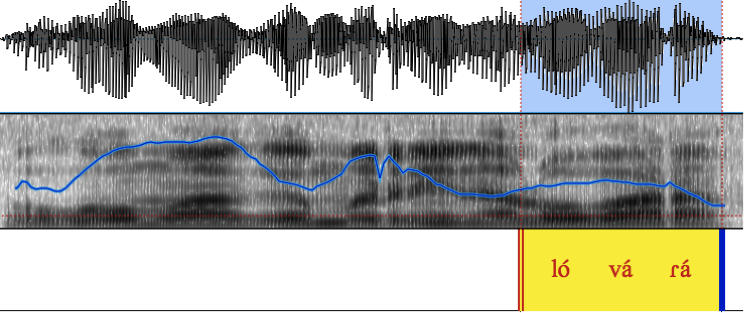
\includegraphics[width=\linewidth]{figures/fig-ch4-1.png}
  \caption{\textit{ogómá gɜmə́rniniə lóvárá} ‘the thief is acting like a guinea fowl.’}
  \label{fig:4-1}
\end{figure}

Words with sequences of LL are pronounced with downdrift, where there is a gradual lowering of f0 across the word, but no sharp fall.

\begin{figure}
  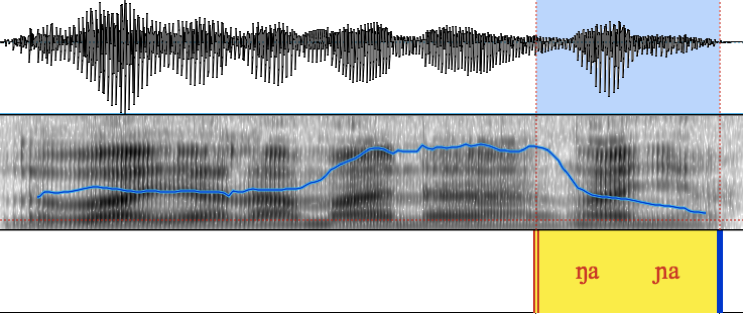
\includegraphics[width=\linewidth]{figures/fig-ch4-2.png}
  \caption{\textit{ləvaja lamáná ŋaɲa} ‘the poor people are cooking grass’}
  \label{fig:4-2}
\end{figure}

Falling tones are also observed with the affixes \textit{-lo} (3pl), \textit{-ja} (inst) and \textit{-u} (loc) which attach at the end of verbs. In general, these affixes cause a H tone to be inserted on the previous syllable if it is otherwise low, as in the following forms:

\ea
\begin{tabular}[t]{ll}
kɜd̪ɜ́t̪ːurt̪iə 	&	‘he’s waiting for it’\\
kɜd̪ɜ́t̪ːurt̪iá\textbf{-lo} 	&	‘he’s waiting for them’\\
katóŋóðeá\textbf{-ja} 	&	‘he’s taking care of it’\\
\end{tabular}
\z

When the previous syllable is a single H tone, however, a falling tone occurs on the suffix:

\ea
\begin{tabular}[t]{lll}
g-a-lat̪-ó 		&	[galat̪ó]	&	‘he molded it’\\
g-a-lat̪-ə́-lo 	&	[galat̪ə́lô]	&	‘he molded them’\\
\end{tabular}
\z

When the verb forms have a sequence of H tones preceding, there is no falling tone, and the suffixes are low-toned. 
\ea
\begin{tabular}[t]{ll}
g-a-lát̪-á 		&	‘he is molding it’ \\
g-a-lát̪-á-lo 	&	‘he is molding them’ \\
t̪úŕt̪-ú			&	‘wait for it!’ \\
t̪úŕt̪-ə́-lo 		&	‘wait for them! \\
\end{tabular}
\z

\section{Tone distribution}\label{sec:ch4:tonedist}
The tone patterns of nouns and verbs are different. Nouns show a range of different high and low lexical sequences. Verb roots do not contrast for lexical tone. Instead, grammatical tone is imposed on verb stems. We will leave discussion of verb tone for the verb section X when aspect, mood and deixis are outlined. 

In the noun system, the main restriction on tone distribution is that two high tones separated by a low cannot occur within a single root (including noun class markers). Exceptions to this are reduplications, such as \textit{ləɲáləɲá} ‘sandstone’. Adjacent sequences of H tone are possible, and the restriction can therefore be analyzed as one single autosegmental H tone per word, assuming that tone sequences consist of a single H tone that is spread to other vowels. The tone patterns observed are as follows.

\ea
\begin{tabular}[t]{llll}
LL	&	&	HH \\\hline
nala	&	'grinding stones'	&	ðáɾá	&	'rope'\\
ləmbi	&	'loincloth'			&	léɲá	&	'egg, penis'\\
oða		&	'deer sp.'			&	ɜ́dí		&	'skin'\\
abəl	&	'bird sp. that hangs upside down'	&	ðə́wáð	&	'buffalo'\\
&\\
LH	&	&	HL\\\hline
ləbú	&	‘well’	&	óna		&	‘small basket’\\
ŋusí	&	‘chick’	&	ðóla		&	‘rat’\\
ɜðú		&	‘breast’&	lóloŋ	&	‘string’\\
ɲogə́l	&	‘eagles’&	élːe	&	‘feather’\\
\end{tabular}
\z

The HL pattern is not as common as the others, and it is often associated with an initial heavy syllable. The LH pattern is also commonly found when the final syllable is heavy. However, as can be seen by the examples, this is a tendency rather than a requirement.

Three syllable words have all possible combinations of L and H except for the unattested HLH. Those of the form HLL, HHL and LHL are less common than the others. This suggests a tendency to favor high tone spreading to the end of the word (Jenks \& Rose 2011). 

\ea
\begin{supertabular}[t]{lllp{3.5cm}}
LLL	&	&	HHH\\\hline
ðəvəra	&	‘line’	&	ðə́bʷáðá	&	'incense-producing tree’\\
ebamba	&	'drum’	&	ɜ́mə́ðíə	&	'celebration'\\
laməɾeð	&	‘non-poisonous snake sp.' &	lə́ŋɡə́ŋé	&	‘bell’\\
&\\
LHH	&	&	LLH\\\hline
ðəbéɾá	&	‘cotton’	&	ðəbəgí	&‘animal trap weighted with a large flat stone’\\
ɜðúní	&	‘hearthstone, oven’	&	ɜgəðiə́	&	'mill floor'\\
lambálá	&hut, shelter	&	ləbopwá	&	‘mushroom’\\
&\\
HLL	&	&	LHL\\
ðɜ́ŋguri	&	‘chameleon’	&	ðəgívi	&	‘bread’\\
ógəŋːa	&	'plant that causes itching'	&	ɜt̪úlɜ	&	‘big spear’\\
áveja	&	'spring, rainy season'	&	lat̪óra	&	‘tomato’\\
&\\
HHL	&	&	HLH\\\hline
ðáŋála	&	‘ewe’	&	$\star$ &\\
lə́búŋwɜ	&	‘water pot, bottle’& &\\
\end{supertabular}
\z

As for words longer than three syllables, similar patterns are found, but again, words with a single H anywhere but the final position are rare. 

\ea
\begin{tabular}[t]{lll}
HHHH	&	ŋə́vándə́ŋé	&	‘type of dried fruit’\\
		&	ɜ́rtə́ŋə́tiə	&	‘armpit’\\
LLLL	&	ŋəmɜgəniə	&	‘work, job’\\
		&	ðabəlat̪a	&	‘thatching tool for smoothing’\\
LHHH	&	ləpə́ndóŋwá	&	‘bushbaby’\\
		&	ŋat̪ábə́lá		&	‘small lock’\\
LLHH	&	lamatáɾá	&	‘support pole’\\
		&	ðəgəmə́níə	&	‘sesame granary’\\
LLLH	&	ed̪apəgá		&	‘nail’\\
		&	ebambəɲá	&	‘skull, eggshell’\\
LLHL	&	ŋavəléka	&	‘mule’\\
		&	aləŋgréma	&	‘bed’\\
LHLL	&	ɜlbɜ́mbɜɾiə	&	‘stool’\\
		&	ləŋɡə́lːəme	&	‘pen, crab’\\
LHHL	&	aɾʧə́ŋála		&	‘broken piece of gourd’\\
		&	aʧóŋgwáɾa	&	‘black bird of prey’\\
HHLL	&	lə́fːə́ɾəŋeə	&	‘bird sp’\\
\end{tabular}
\z

\section{Tone spreading}
There are four tonal spreading rules in Moro, two in the nominal system and two associated with verbs.

In the nominal system, a H tone spreading rule is observed with the instrumental/comitative suffix \textit{-Ca}. The C indicates that the consonant agrees in noun class (Jenks \& Rose 2011). The tone of the suffix matches that of the final syllable of the noun. This can be analyzed as tone spreading from the noun stem to the suffix. 

\begin{table}
\caption{Instrumental –Ca}
	\begin{tabular}[t]{llllll}
		Final H & & &  Final L\\\hline
LH-H	&	ɜðú-já	&	‘breast'	&	LL-L		&	eða-ɡa	&	‘meat’\\
HH-H	&	ŋíní-ŋá	&	‘dog’	&	HL-L		&	ðót̪oŋ-ða	&	‘agama lizard’\\
LLH-H	&	ðəŋəlá-ðá	&	‘tongue’	&LLL-L	&	ðamala-ða	&	‘camel’\\
LHH-H	&	ðəbáɾá-ðá	&	‘cotton’		&	HLL-L	&	áveja-ga	&	‘spring’\\
HHH-H	&	ŋə́və́ní-ŋá		&	‘blood’		&	LHL-L	&	padóla-ða	&	‘jute’ \\
	\end{tabular}
  \label{tab:ch4:2}
\end{table}

The locative prefix \textit{é-} (allomorphs: í, ék-, és-, ég-, ík, ís-, íg-) spreads high tone rightwards. There are two possible variants of this rule. Either the high tone may spread once to the following syllable, or it may spread to the end of the noun stem (excluding other suffixes), as shown below. In both cases, if the noun contains a LH sequence, H tone spreading halts one syllable away to avoid placing two H tones adjacent to teach other, ex. \textit{ðəŋəlá  é-ðə́ŋəlá}.

\begin{table}
	\begin{tabular}[t]{llllll}
Noun	&	locative		&	&			Noun		&	locative		&	\\\hline
ðaba	&	é-ðábá		&	cloud	&	ðəŋəlá	&	é-ðə́ŋəlá		&	tongue\\
ðamala	&	é-ðámálá	&	camel	&	ogovélá	&	ék-ógovél	&	monkey\\
ŋíní 	&	í-ŋíní		&	dog		&	ðót̪oŋ 	&	é-ðót̪oŋ		&	agama lizard\\
ŋə́və́ní	&	í-ŋə́və́n		&	blood	&	áveja	&	ék-áveja		&	spring\\
ŋə́ðə́máná	&	é-ŋə́ðə́mán		&	beans	&	ðáŋála	&	é-ðáŋála	&	sheep\\
etám	&	ég-ətám		&	neck		&	eváɾt̪ə́ŋé	&	ék-əváɾt̪ə́ŋ	&	type of tree\\
ðəbáɾá	&	é-ðəbáɾá	&	cotton	&	ləŋɡɜ́lːəme	&	é-ləŋɡɜ́lːəme	&	pen\\
padóla	&	é-padóla	&	jute		&	aʧóŋgʷára	&	ég-aʧóŋgʷár	&	‘bird of prey’\\
	\end{tabular}
	\caption{Locative é-}
	\label{tab:ch4:3}
\end{table}

The addition of this prefix can condition loss of the final vowel. See details of this prefix in section X.

In the verbs, there are two patterns of H tone spreading. One involves H tone on the stem in proximal imperfective and dependent clause verb forms. The second involves H tone spread from a final perfective vowel to a following object. 

If a verb root is of the shape CVC, H tone appears on the root in the proximal imperfective and in dependent clause forms. This H tone is spread or extended one syllable to the right for most verbs. This is typically to the final aspect suffix, \textit{-a} or \textit{-eə} (or vowel harmony variants [ɜ], [iə]). 

\ea
\begin{tabular}[t]{llll}
H-H pattern		&				&	H-L pattern		&	\\
g-ɜ-sɜ́ð-ɜ́		&	‘defecate’	&	g-a-tóð-a		&	‘move’\\
g-a-wáð-á		&	‘poke’		&	g-a-váð-a 		&	‘shave’\\
g-a-nát̪-á		&	‘taste’		&	g-a-sát̪-a		&	‘chew’\\
g-a-bwáɲ-á		&	‘like, wantʼ	&	g-a-nwán-a		&	‘watch’\\
\end{tabular}
\z

However, if the passive, anti-passive or benefactive applicative suffix appears before the final aspect suffix, it will host the H tone. This is the case with both kinds of short verbs:

\ea
\begin{tabular}[t]{llll}
	&	Imperfective	&	Imperfective passive &	\\
H-H &	g-a-bwáɲ-á		&	g-ɜ-bwɜ́ɲ-ə́n-iə		&	‘like, want’\\
	&	g-a-wáð-á	&	g-ɜ-wɜ́ð-ə́n-iə		&	‘poke’\\
H-L	&	g-a-váð-a	&	g-ɜ-vɜ́ð-ə́n-iə		&	‘shave’\\
	&	g-a-tóð-a	&	g-ɜ-túð-ə́n-iə	&	‘move’\\
\end{tabular}
\z

If a perfective verb is followed by an object beginning with a low tone, H tone spreads from the perfective to the following object, as in (19)c,d:

\ea
\begin{xlist}
	\ex \gll l-a-mámː-atʃəð-a ŋavəɾa\\
			\textsc{sm}.\textsc{cl}l-\textsc{rtc}-\textsc{iter}-take-\textsc{recip}-\textsc{impv} \textsc{cl}ŋ.stick\\
			\trans	‘they are taking sticks from each other’
	\ex \gll l-a-pə́g-á 	lugi 	loaɲa\\
			\textsc{sm}.\textsc{cl}l-\textsc{rtc}-uproot-\textsc{impv} \textsc{cl}l.tree	\textsc{cl}l.many\\
			\trans	‘they are uprooting a lot of trees’
	\ex \gll	l-a-mː-atʃəð-ó 				ŋávəɾa\\
			\textsc{sm}.\textsc{cl}l-\textsc{rtc}-take-\textsc{recip}-\textsc{pfv}		\textsc{cl}ŋ.stick\\
			\trans	‘they took sticks from each other’
	\ex \gll l-a-pəg-ó 	lúgi 	loaɲa\\
			\textsc{sm}.\textsc{cl}l-\textsc{rtc}-uproot-\textsc{pfv}	\textsc{cl}l.tree	\textsc{cl}l.many\\
			\trans	‘they uprooted a lot of trees’
\end{xlist}
\z

Other verb forms that have already undergone H tone spreading within the verb stem, such as the imperfective, do not condition this cross-word spreading (19)b.

As all these examples involve restrictions on H tone or H tone spreading, and contour tones do not appear phonologically, Jenks \& Rose (2011) analyze Moro as a H/0 tone system where low tone is not specified with an autosegmental tone. In all cases of high tone spreading, it is in the progressive or rightward direction. There are no observed cases in the language of high tone spreading leftwards. 

\section{Downstep}
Downstep, or the lowering of a H tone adjacent to another H tone, is observed at some word and stem boundaries in Moro. H tones do not generally delete, but they can lower.

The perfective high tone spreading rule discussed in section 4.4 does not apply if the following noun begins with a high tone. In this case, downstep occurs on the object.

\ea
\begin{xlist}
	\ex
	\gll	l-a-pəg-ó 	$^{\downarrow}$nə́deə́	 noaɲa\\
		\textsc{sm}.\textsc{cl}l-\textsc{rtc}-uproot -\textsc{pfv}	\textsc{cl}n.doleib palm 	\textsc{cl}n.many\\
	\trans ‘they uprooted a lot of doleib palm trees’
	\ex
	\gll	ŋerá	ŋalagó 		$^{\downarrow}$ŋwóréðá\\		
		\textsc{cl}ŋ.girl	\textsc{sm}.\textsc{cl}ŋ-\textsc{rtc}-plant-\textsc{pfv}	\textsc{cl}ŋ.sesame seed\\	
	\trans ‘the girl planted sesame seeds’
\end{xlist}
\z

This can be seen in the following sentence in which the HHH object \textit{ŋwóɾéðá} shows a drop of the H tones to a mid f0 range following the final H of the verb, but not as low as the low tones of the verb \textit{ŋalagó} preceding it. The final syllable of the sentence shows a falling tone as discussed above.

\begin{figure}
  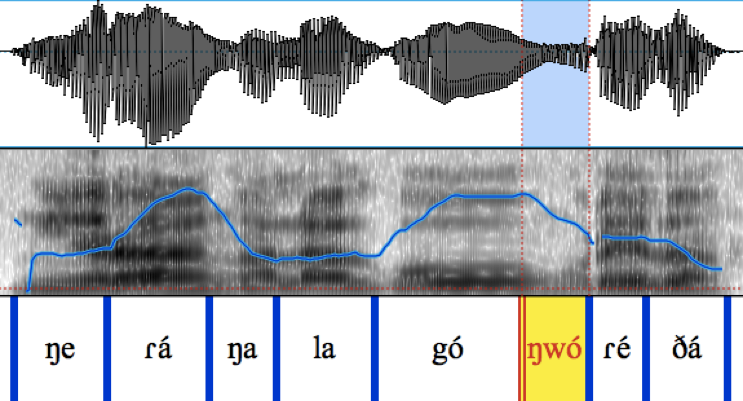
\includegraphics[width=\linewidth]{figures/fig-ch4-3.png}
  \caption{\textit{ŋerá ŋalagó ŋwóréðá} ‘the girl planted sesame seeds’}
  \label{fig:4-3}
\end{figure}

The other environments for downstep occur within the verb stem. 

\section{Tone stability}
Moro shows tonal stability. If a vowel bearing a single H tone is deleted, the H tone appears on a neighboring vowel or sonorant, a phenomenon referred to as tonal stability Tonal stability occurs when vowels are juxtaposed across morphemes or word-boundaries, and the first vowel deletes. Compare the forms in (a) and (b). In the latter, the subject relative clause marker \textit{é-} is deleted due to the following vowel-initial root, but its high tone appears on the [o] of the root. In (d), the object marker \textit{ɲé-} loses its vowel, and the high tone is recuperated on the preceding vowel rather than the following, a pattern which appears to be unique to high-toned object markers. 

\ea
\begin{tabular}[t]{lll}
g-a-ogət̪-ó	&	[kogət̪ó]	&	‘s/he jumped’\\
g-é-ogət̪-ó	&	[kógət̪ó]	&	‘…. who (sg.) jumped’\\
g-ɜ-ɜwut̪-ɜ	&	[kɜwút̪ɜ]	&	‘he is about to drop something’\\
g-ɜ-ɲé-ɜwut̪-ɜ&	[kɜ́ɲɜwut̪ɜ]	&	‘he is about to drop me’\\
\end{tabular}
\z

In each case, however, the high tone appears on another host.

In running speech, the same effect is observed across word boundaries:

\ea	lapəgúgi\\
	\gll l-a-pəg-ó ugi 	 \\
	\textsc{sm.cll}-\textsc{rtc}-uproot-\textsc{pfv}	 clg.tree	 \\
	\trans ‘they are uprooting tree’
\z

\section{Intonation}
Moro employs intonation to convey distinctions between polar (yes/no) questions and declarative statements as well as utterance continuations and focus/cleft constructions. Intonation interacts with the lexical tone of the utterance, but in a circumscribed manner. In general, the lexical tones are maintained and the entire pitch range or register is raised. Word-final utterance position, however, exhibits pitch compression and declination, even in questions. 

Declarative utterances and yes/no questions (those to which the response is yes or no) are distinguished by i) a question particle and ii)  pitch raising. Yes/no questions are often marked with an \textit{-a}, which attaches to the final word in the question. However, the particle is optional, and is not obviously present on words than end in [a]. The two types of utterances are otherwise distinguished by pitch. Yes/no questions show raised pitch in the early part of the utterance, with lower pitch during the rest of the utterance, especially on the final word. Speakers differ in whether the final fall in pitch occurs over the whole final word or is confined to the final syllable. 
Consider the following two pitch tracks, showing the F0 (fundamental frequency), which is the acoustic measurement for tone. The first utterance is a declarative sentence [lɜmːiə lalágá ŋwala] 'the boys are about to plant sesame seeds' and the second a polar question with the same words, both uttered by Angelo Naser. As can be seen in the first pitch track, the pitch raises for the high tones in the declarative sentence, and there is a fall at the end, so the final syllable of the utterance is the lowest point. \begin{figure}
  \includegraphics[width=\linewidth]{figures/declarativeintonation.pdf}
    \label{fig:4-4}
\end{figure}

In the polar question, the sentence starts slightly higher, but the main distinction is that the lexical high tone targets are significantly raised to about 220Hz, whereas they are at about 150Hz in the declarative. The final low-toned, word, however, is articulated in a similar manner to that in the declarative sentence. Questions do not show final rising intonation in Moro, a pattern which is attested in a number of other African languages (Rialland 2007). 
Another example illustrates the same pattern, this time articulated by Elyasir Julima. In this example, all the words have high tones: ŋeɾá ŋalagó ŋwóréðá 'the girl planted sorghum seeds'. Note that the final word which has three high tones, shows downstep (a lower H tone) following the final high of the verb, with gradual declination. 

\begin{figure}
  \includegraphics[width=\linewidth]{figures/declarativeintonation2.pdf}
\label{fig:4-4}
\end{figure}

In the question version of the same sentence, the first high tone of the utterance shows slightly higher pitch  compared to the declarative, but all the following high tones showing tonal compression. In particular the LLH lexical tone of the second word exhibits tone flattening. Again, the utterance shows declination at the end, so that the HHH word resembles a LLL word. 
\begin{figure}
  \includegraphics[width=\linewidth]{figures/questionintonation2.pdf}
\label{fig:4-4}
\end{figure}


Consider the following two utterances and the pitch tracks associated with them. The higher (black) pitch track is a yes/no question, and the lower (red) pitch track is the declarative utterance. The two utterances are identical in terms of segments and lexical tones, but differ in overall pitch. The question has higher pitch targets than the declarative in the early part of the utterance, although both fall in utterance final position. This shows that questions do not show final raising. The tone peak represents both H tones on \textit{máná}

\begin{figure}
  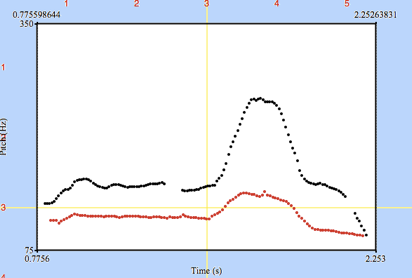
\includegraphics[width=\linewidth]{figures/fig-ch4-4.png}
  \caption{\gll ləvaja     l-a-mán-á                       ŋaɲa\\
\textsc{cl}l.poor \textsc{sm.cll}-\textsc{rtc}-cook-\textsc{impv} \textsc{cl}ŋ.grass\\
\trans Black = question, Red = declarative}
  \label{fig:4-4}
\end{figure}

This example is similar, but each word has H tones, and each of the H tone peaks are higher in the question version of the utterance.

\begin{figure}
  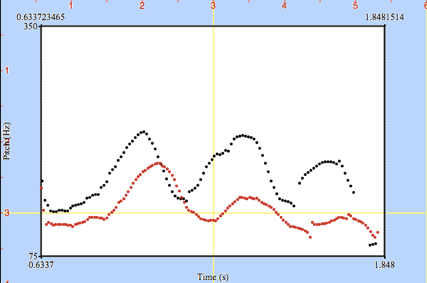
\includegraphics[width=\linewidth]{figures/fig-ch4-5.png}
  \caption{\gll ŋəməná ŋamə́nwá ŋgárá\\
\textsc{cl}ŋ.baby goat \textsc{sm}.\textsc{cl}ŋ-\textsc{rtc}-lick-\textsc{impv} \textsc{cl}ŋ.salt\\ \trans }
  \label{fig:4-5}
\end{figure}

% TODO Question MORE NEEDED ON INTONATION